\section{Overview}
There exists a whole class of methods, all of which called the kernel polynomial method, or KPM for short.
They are powerful tools for approximating the spectral density of matrices.
We will focus on the main approach in the following.\\
As the name suggests, the KPM is a polynomial extension of the spectral density.
The coefficients of the polynomials are derived from the method of moments,
in order to obtain an estimator function as in statistics.

The method is based on a corollary of the following generalized theorem:

\begin{theorem}
    Let $A \in \C^{n \times n}$ be a normal matrix with spectral decomposition
    \[
    A = U \Lambda U^* \quad \text{where} \quad UU^* = I_n \text{ and } \Lambda = \diag(\lambda_1, ..., \lambda_n)
    \]
    Let $\beta, v \in \C^n$ with $v = U\beta$.
    Suppose $v$ is a random vector whose entries $v_i$ are independent and identically distributed standard complex normal variables,
    i.e., $v_i \sim_\text{i.i.d.} \mathcal{N}_\C(0, 1)$, meaning $\Real(v_i), \Imag(v_i)$ are independent $\mathcal{N}(0, \frac{1}{2})$.
    Then
    \begin{equation} \label{eq:complex_normal_vector}
        \E[v] = 0 \quad \text{and} \quad \E[v v^*] = I_n,
    \end{equation}
    and it follows that
    \[
    \E[\beta] = 0 \quad \text{and} \quad \E[\beta \beta^*] = I_n.
    \]
\end{theorem}


\begin{proof}[Proof of Theorem 1]
    Since the expectation operator is linear, it holds that
    \[
    \E[v] = \E[U\beta] = U\E[\beta] = 0 \implies \E[\beta] = 0
    \]
    Furthermore it holds that
    \[
    I_n = \E[vv^*] = \E[(U\beta)(U\beta)^*] = \E[U\beta \beta^*U^*] = U \E[\beta \beta^*]U^*
    \]
    Multiplying both sides with $U^*$ and $U$ yields:
    \[
    U^* I_n U = U^* U \E[\beta \beta^*]U^* U = \E[\beta \beta^*]
    \]
    Since $U$ is unitary, we have shown that $\E[\beta \beta^*] = I_n$.
\end{proof}


\vspace{0.5 cm}
This theorem has a nice corollary when investigating a matrix function $f(A)$.
In that case, we have

\begin{align*}
    \E\left[v^* f(A) v\right] &= \E\left[(U\beta)^* f(U\Lambda U^*) (U\beta)\right] \\
        &= \E\left[\beta^* U^* U f(\Lambda) U^* U \beta\right] \\
        &= \E\left[\beta^* f(\Lambda) \beta\right] \\
        &= \E\left[\sum_{j = 1}^n |\beta_j|^2 f(\lambda_j) \right] \\
        &= \sum_{j = 1}^n f(\lambda_j) \E\left[ |\beta_j|^2 \right] \\
        &= \sum_{j = 1}^n f(\lambda_j)
\end{align*}

or, more concisely,
\begin{equation} \label{eq:theorem_result}
    \E\left[v^* f(A) v\right] = \Tr(f(A)).
\end{equation}

We now have a method to calculate the trace of a matrix function $f(A)$,
using only vector multiplications with $A$.

\section{Polynomial Extension with Chebyshev polynomials}
We assume Chebyshev polynomials to be a good fit for the polynomial extension of the Dirac delta distribution
because of the many great properties we will see now. First, let's look how Chebyshev polynomials are defined.
Using the trigonometric functions, they can be expressed as follows:

\[ T_k(x) =
\begin{cases}

\cos(k \arccos(x))                & \quad \text{for } k \in [-1, 1]\\
    \cosh(k \arcosh(x))           & \quad \text{for } k > 1\\
    (-1)^k \cosh(k \arcosh(-x))   & \quad \text{for } k < -1
\end{cases}
\]

We will only use the formula $T_k(x) = \cos(k \arccos(x))$.
This means to only consider matrices, which have eigenvalues within the intervall $[-1, 1]$.
In the case that this condition should not be fulfilled, the eigenvalues can be transformed accordingly.
For this, let $\lambda_{lb}$ and $\lambda_{ub}$ be the lower and upper bound for the eigenvalues of $A$, respectively.
To find these, well-established methods like the Gershgorin circle theorem can be used.

Define
\[
c := \frac{\lambda_{lb} + \lambda_{ub}}{2} \quad \text{and} \quad d := \frac{\lambda_{ub} - \lambda_{lb}}{2}
\]
Then, the matrix $B = \frac{A - c*I_n}{d}$ has eigenvalues in the interval $[-1, 1]$.
A visualization of this is linked in the appendix.


Another way to define Chebyshev polynomials is by calculating them using the recursion formula
\[
T_{k + 1}(x) = 2xT_k(x) - T_{k - 1}(x),
\]
where the starting conditions are given by $T_0(x) = 1$ and $T_1(x) = x$.

Additionally, note that the result in equation \ref{eq:theorem_result} says, that

\begin{equation} \label{eq:Chebyshev_trace}
    \E\left[\,v^T T_k(A) v\,\right] = \Tr\left(T_k(A)\right).
\end{equation}

This result will be central in the following discussion.


Now, let
\begin{equation} \label{eq:weight_function}
    h(x) = \frac{1}{\sqrt{1 - x^2}}
\end{equation}
be a weight function.
Another property of Chebyshev polynomials is
that they are \emph{orthogonal} in terms of the scalar product weighted with $h$:

\[
\left \langle f, g \right \rangle = \int_{-1}^1 \frac{1}{\sqrt{1 - x^2}} \cdot f(x) \cdot g(x) \dx.
\]

This means that

\[
\int_{-1}^1 \frac{1}{\sqrt{1 - t^2}} \cdot T_k(t) \cdot T_l(t) \dt =
\begin{cases}
    0               & \quad \text{for } k \neq l\\
    \pi             & \quad \text{for } k = l = 0\\
    \frac{\pi}{2}   & \quad \text{for } k = l \neq 0
\end{cases}
\]

\section{Approximating the spectral density}
Now multiply the spectral density with the inverse of the weight function \ref{eq:weight_function}:
\[
\hat{\phi}(x) = \sqrt{1 - x^2} \phi(x) = \sqrt{1 - x^2} \, \cdot \, \frac{1}{n} \sum_{j = 1}^n \delta(x - \lambda_j)
\]
Let $g \in \SR$, the Schwartz space defined in definition \ref{def:Schwartz space},
and $\mu_k \in \R$ coefficients to be determined such that the following equation holds:

\begin{equation} \label{eq:distribution_equality}
    \int \limits_{-1}^1 \hat{\phi}(t) g(t) \dt = \int \limits_{-1}^1 \sum_{k = 0}^{\infty} \mu_k T_k(t) g(t) \dt
\end{equation}

If this is true for arbitrary $g \in \SR$, we can simplify our equation \ref{eq:distribution_equality} to

\begin{equation} \label{eq:Chebyshev-Expansion}
    \hat{\phi}(x) = \sum_{k = 0}^{\infty} \mu_k T_k(x)
\end{equation}


Now utilize the orthogonality of the Chebyshev polynomials, to calculate a specific coefficient $\mu_k$:

\begin{align*}
    & \; \; \sum_{l = 0}^{\infty} \mu_l T_l(t) = \hat{\phi}(t) \\
    \implies & \left(\sum_{l = 0}^{\infty} \mu_l T_l(t)\right) \cdot T_k(t) = \hat{\phi}(t) \cdot T_k(t)\\
    \implies & \int_{-1}^1 \frac{1}{\sqrt{1 - t^2}} \cdot \left(\sum_{l = 0}^{\infty} \mu_l T_l(t)\right) \cdot T_k(t) \dt = \int_{-1}^1 \frac{1}{\sqrt{1 - t^2}} \cdot \hat{\phi}(t) \cdot T_k(t) \dt\\
    \implies & \mu_k \cdot \frac{\pi}{2 - \delta_{k0}} = \int_{-1}^1 \frac{1}{\sqrt{1 - t^2}} \cdot \sqrt{1 - t^2} \cdot \phi(t) \cdot T_k(t) \dt\\
    \implies & \mu_k = \frac{2 - \delta_{k0}}{\pi} \cdot \int_{-1}^1 \phi(t) \cdot T_k(t) \dt\\
\end{align*}

By applying the Dirac delta distribution we obtain:
\begin{align*}
    \mu_k = \frac{2 - \delta_{k0}}{\pi} \cdot \int_{-1}^1 \phi(t) \cdot T_k(t) \dt &= \frac{2 - \delta_{k0}}{\pi} \cdot \int_{-1}^1 \frac{1}{n} \sum_{j = 1}^n \delta(t - \lambda_j) \cdot T_k(t) \dt \\
    &= \frac{2 - \delta_{k0}}{n \pi} \sum_{j = 1}^n T_k(\lambda_j)\\
    &= \frac{2 - \delta_{k0}}{n \pi} \Tr(T_k(A))
\end{align*}

Now let $n_{\text{vec}} \in \R$ and consider vectors $v_0^{(1)}, v_0^{(2)}, \dots, v_0^{(n_{\text{vec}})}$,
which are chosen randomly from the standard normal distribution,
that is to say $\E[v_0^{(k)}] = 0$ und $\E\left[v_0^{(k)}\left(v_0^{(k)}\right)^T\right] = I_n$.
It follows from equation \ref{eq:Chebyshev_trace} that
\[
\zeta_k = \frac{1}{n_{\text{vec}}} \sum_{l = 1}^{n_{\text{vec}}} \left( v_0^{(l)} \right)^T T_k(A) v_0^{(l)}
\]
is a good estimator for $\Tr(T_k(A))$ and therefore
\[
\mu_k \approx \frac{2 - \delta_{k0}}{n \pi} \zeta_k
\]

In order to determine the $\zeta_k$, let $v_0 \equiv v_0^{(l)}$
Using the recursion formula for Tschebyschev polynomials, we can calculate
\[
T_{k + 1}(A)v_0 = 2 A T_k(A) v_0 - T_{k - 1}(A) v_0
\]
For $v_k \equiv T_k(A)v_0$ it also holds that
\[
v_{k + 1} = 2 A v_k - v_{k - 1}
\]

With this we are fully equpped for the final calculation and the goal of the KPM is reached:
Instead of having to multiply matrices with other matrices, it now suffices to multiply matrices with vectors.
Now we can approximate $\phi(x)$ as closely as we like.
As aforementioned, it is not always desirable to have an infinitely exact approximation.
Since it holds that
\[
\lim \limits_{k \to \infty} \mu_k \to 0
\]
and we are only interested in $T_k(x)$ with $k \leq M$\\
Therefore we estimate $\phi$ with
\begin{equation} \label{eq:Angenäherte Spektraldichte}
    \tilde{\phi}_M(x) = \frac{1}{\sqrt{1 - x^2}} \sum_{k = 0}^{M} \mu_k T_k(x)
\end{equation}

The following pseudo code is based on \cite[p.~10]{linsaadyang14} and summarizes the steps described above.
The implementation is done in Python, and linked in the appendix.

\begin{algorithm}
    \caption{The Kernel Polynomial Method}\label{alg:cap}
    \begin{algorithmic}[5]
    \Require $A = A^* \in \mathbb{C}^{n \times n}$ with eigenvalues in the intervall $[-1, 1]$
    \Ensure Estimated spectral density \{$\tilde{\phi}_M(t_i)$\}\\
    \For{$k = 0 : M$}
    \State $\zeta_k \gets 0$
    \EndFor
    \For{$l = 1 : n_{\text{vec}}$}
    \State $\text{Choose a random new vector } v_0^{(l)}\text{;}$ \Comment{$v_{0_i}^{(l)} \sim_\text{ i.i.d. } \mathcal{N}(0, 1)$}
    \For{$k = 0 : M$}
    \State $\text{Calculate } \zeta_k \gets \zeta_k + \left( v_0^{(l)} \right)^T v_k{(l)}\text{;}$  
    \If{$k = 0$}
    \State $v_1^{(l)} \gets A v_0^{(l)}$
    \Else
    \State $v_{k+1}^{(l)} \gets 2 A v_k^{(l)} - v_{k-1}^{(l)}$ \Comment{Three term recursion}
    \EndIf
    \EndFor
    \EndFor
    \For{$k = 0 : M$}
    \State $\zeta_k \gets \frac{\zeta_k}{n_{\text{vec}}}$
    \State $\mu_k \gets \frac{2 - \delta_{k0}}{n \pi} \zeta_k$
    \EndFor
    \State $\text{Evaluate } \tilde{\phi}_M(t_i) \text{ with equation } \ref{eq:Angenäherte Spektraldichte}$
    \end{algorithmic}
\end{algorithm}

Applying the Cayley transform to an arbitrary unitary matrix $U$ yields a Hermitian matrix $H$;
and as this is the case, the KPM can be applied to unitary matrices as well.

\section{The Choice of Random Unitary Matrices}

When generating random unitary matrices for numerical experiments,
it is important to ensure that their eigenvalues are distributed uniformly on the unit circle,
as predicted by random matrix theory.
A common approach is to generate a random complex matrix $A$ with independent standard normal entries
and then construct a unitary matrix from $A$ using either the QR decomposition or the singular value decomposition (SVD).
In the QR approach, $A$ is factored as $A = QR$, where $Q$ is unitary and $R$ is upper triangular.
The matrix $Q$ is then used as the random unitary matrix.
In the SVD approach, $A$ is factored as $A = U \Sigma V^*$,
and either $U$ or $V$ (both unitary) can be used as a random unitary matrix.
Although both methods produce unitary matrices, their statistical properties differ.
The SVD-based approach yields unitary matrices whose eigenvalues are uniformly distributed on the unit circle,
matching the theoretical prediction for random unitary matrices (the so-called Haar measure).
In contrast, the QR-based approach does not generally produce a uniform distribution of eigenvalues on the unit circle.
This distinction is important for applications where the spectral properties of random unitary matrices play a central role,
such as in the study of spectral densities.
For such purposes, the SVD-based construction is preferable,
as it ensures the correct statistical behavior of the eigenvalues.

\begin{figure}[htb]
    \centering
    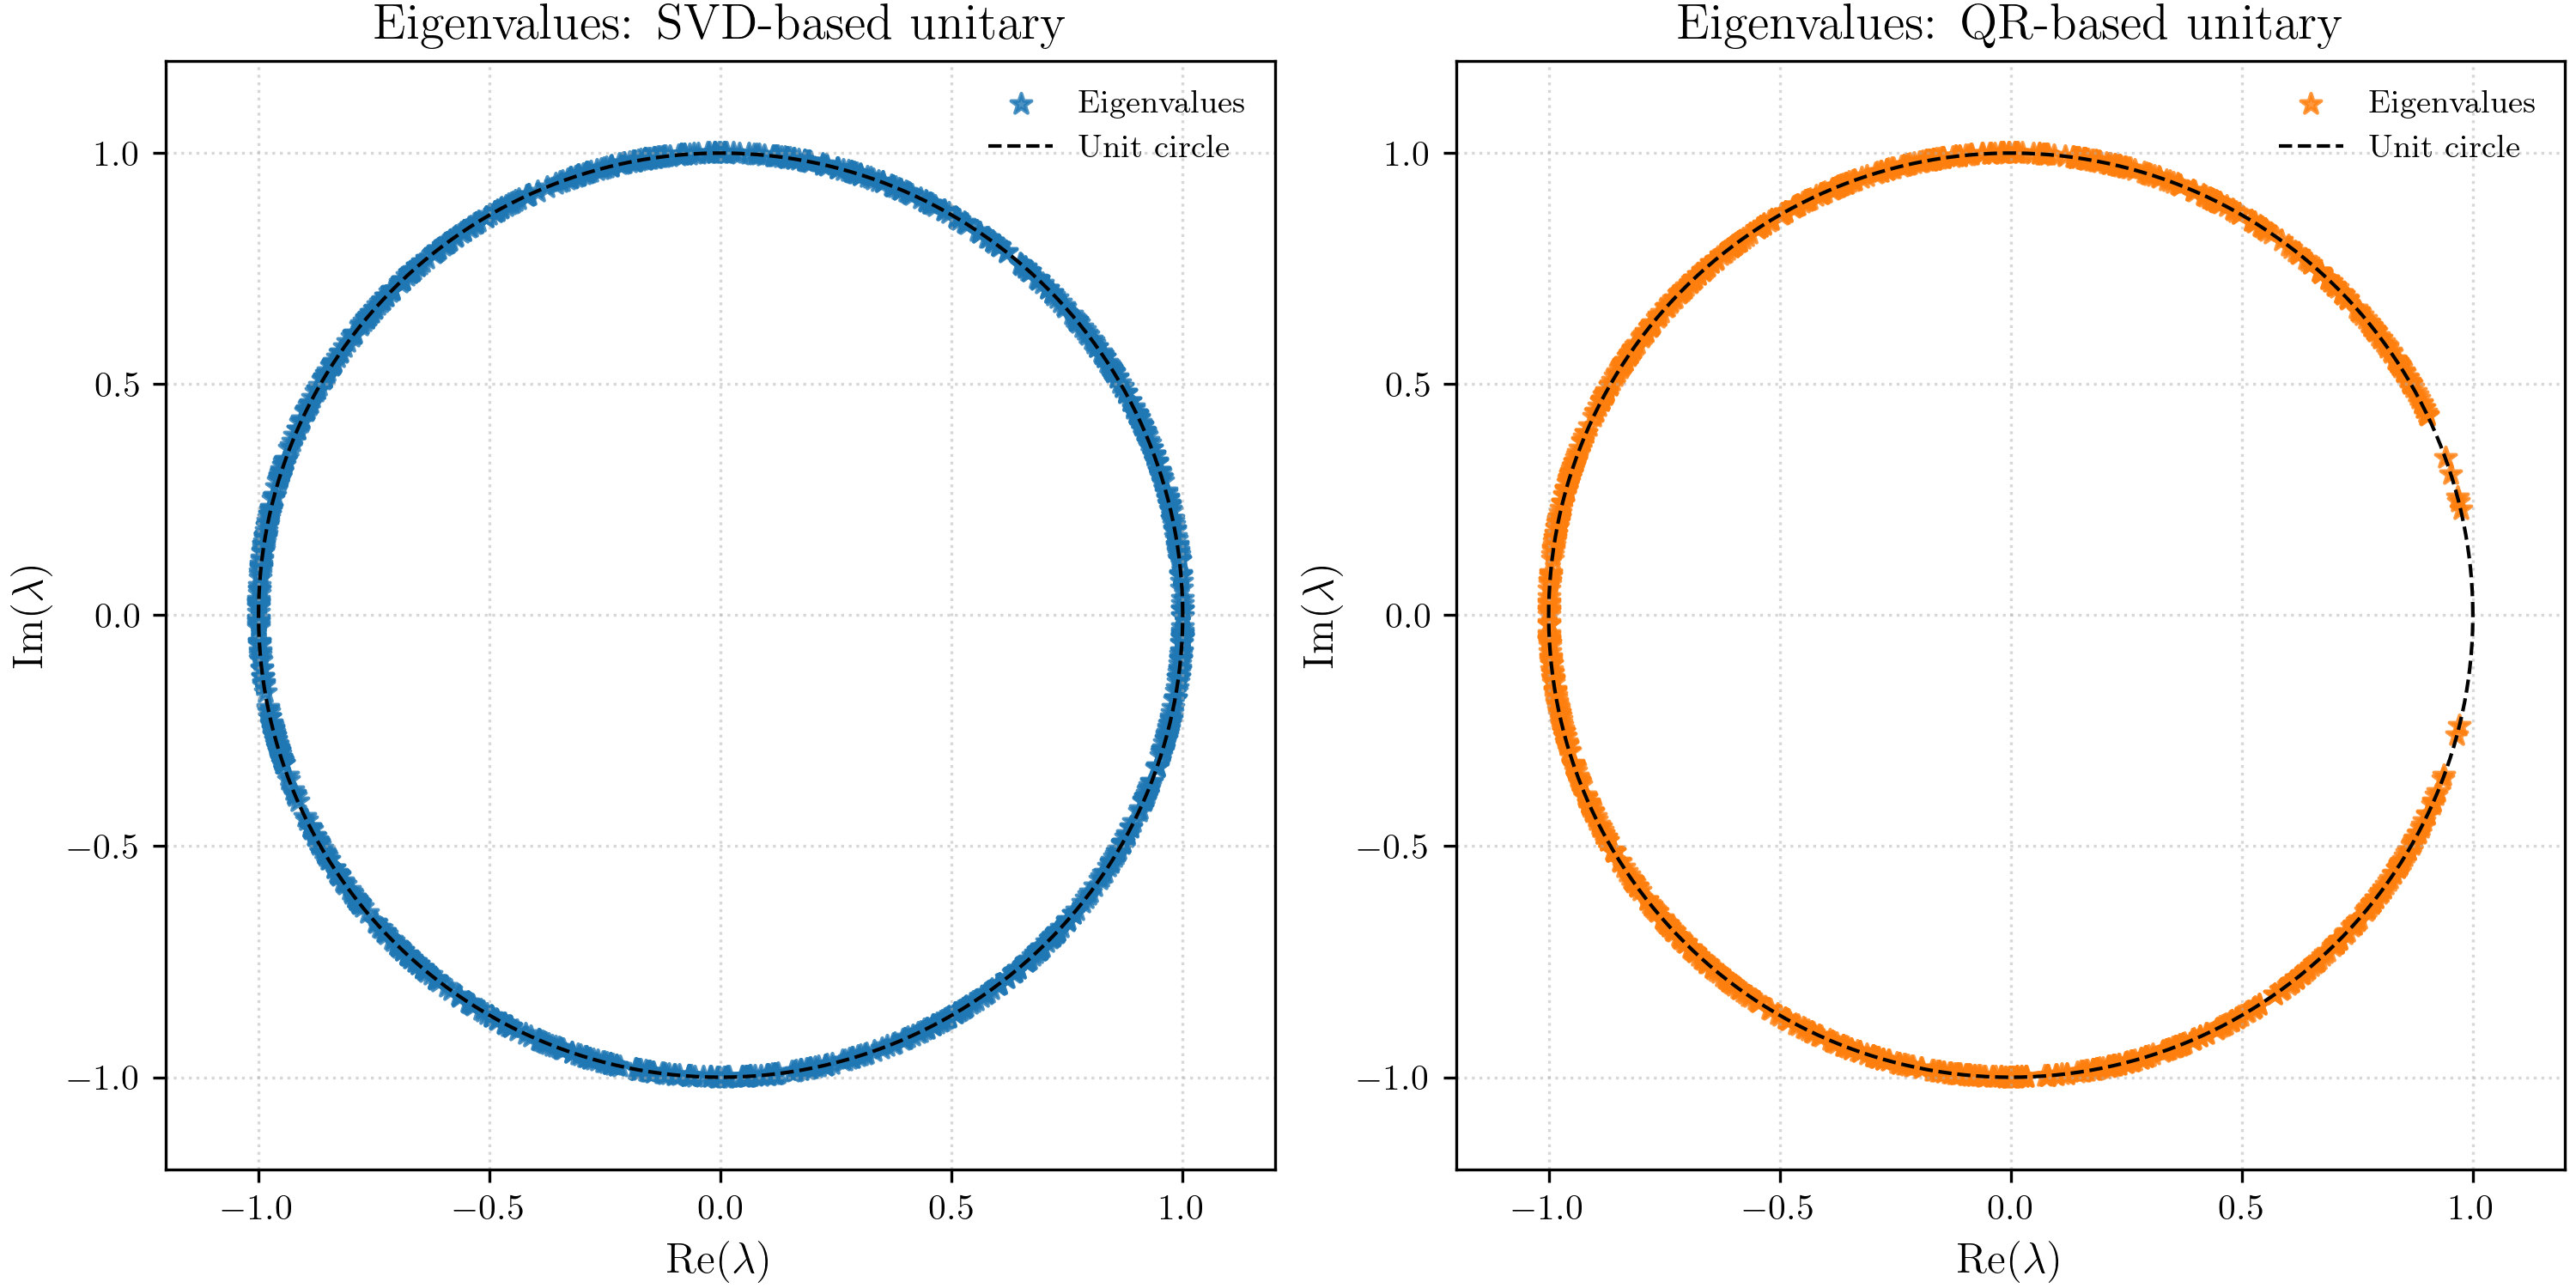
\includegraphics[width=1\textwidth]{Graphics/eigenvalue_comparison.png}
    \caption{Eigenvalue distributions of random unitary matrices generated via SVD and QR.}
    \label{fig:eigenvalue-comparison}
\end{figure}